
\documentclass[conference]{IEEEtran}
\IEEEoverridecommandlockouts
% The preceding line is only needed to identify funding in the first footnote. If that is unneeded, please comment it out.
\usepackage{cite}
\usepackage{amsmath,amssymb,amsfonts}
\usepackage{algorithmic}
\usepackage{graphicx}
\usepackage{textcomp}
\usepackage{booktabs}
\usepackage[procnames]{listings}
\usepackage{xcolor}
\def\BibTeX{{\rm B\kern-.05em{\sc i\kern-.025em b}\kern-.08em
    T\kern-.1667em\lower.7ex\hbox{E}\kern-.125emX}}
\begin{document}

\title{Decoding Performance: A Comparative Analysis of Open-Source Compilers\\
{\footnotesize \textsuperscript{*}CS323 2023F Research Report}
\thanks{}
}

\author{
\IEEEauthorblockN{1\textsuperscript{st} Ruixiang JIANG}
\IEEEauthorblockA{\textit{SUSTech} \\
Shenzhen, China \\
12111611@mail.sustech.edu.cn}
\and
\IEEEauthorblockN{2\textsuperscript{nd} Liquan WANG}
\IEEEauthorblockA{\textit{SUSTech} \\
Shenzhen, China \\
12011619@mail.sustech.edu.cn}
\and
\IEEEauthorblockN{3\textsuperscript{rd} Wenhui TAO}
\IEEEauthorblockA{\textit{SUSTech} \\
Shenzhen, China \\
12111744@mail.sustech.edu.cn}
}
\maketitle

\begin{abstract}
The landscape of open-source compilers is diverse and dynamic, with several prominent players contributing significantly to the field. This research delves into a comprehensive analysis and comparison of five prominent open-source compilers: GCC, Clang, LLVM, Codon, and Ark Compiler (also known as FangZhou). The study aims to elucidate the distinctions among these compilers, focusing on aspects such as architecture, optimization techniques, language support, and overall performance. Additionally, a crucial facet of this investigation involves an in-depth examination of the runtime speed differences exhibited by these compilers. By providing a detailed comparison, this research equips developers and enthusiasts with valuable insights to make informed decisions regarding compiler selection for diverse programming needs.
\end{abstract}

\begin{IEEEkeywords}
Compiler, GCC, Clang, LLVM, Codon, Ark Compiler
\end{IEEEkeywords}

\section{Introduction}
Traditional compilers are typically divided into three main components: the frontend, optimizer, and backend. During the compilation process, the frontend is primarily responsible for lexical and syntactical analysis, transforming source code into an abstract syntax tree. The optimizer builds upon the frontend by enhancing the efficiency of the generated intermediate code through various optimization techniques. The backend then translates the optimized intermediate code into machine code tailored for specific platforms.

These three components collaborate to form the complete workflow of a compiler. The frontend understands the structure and syntax of the source code, creating an intermediate representation. The optimizer improves program performance and efficiency through a series of optimization techniques. Finally, the backend translates the optimized intermediate code into machine code relevant to the hardware platform, enabling the computer to execute the program.

As the demand for efficient and high-performance compilers continues to rise, the open-source community has witnessed the emergence and evolution of several notable compiler projects. In this research, we explore and compare five such compilers that have made significant contributions to the field: GCC, Clang, LLVM, Codon, and Ark Compiler.

GCC (GNU Compiler Collection), stands as one of the most venerable and widely-used open-source compilers, supporting an extensive range of programming languages and platforms. Its robust architecture and comprehensive feature set have solidified its position as a cornerstone in the development community.

LLVM (Low-Level Virtual Machine), serves as a standalone compiler infrastructure, providing a foundation for various language front ends. Its innovative design, featuring an intermediate representation (IR) and a wide range of optimization passes, has enabled LLVM to find applications beyond traditional compiler use cases.

Clang, renowned for its emphasis on modularity and user-friendly design, has gained prominence as a compiler front end, often coupled with LLVM as its backend. Its modular architecture and focus on static analysis have made it an attractive choice for developers seeking a versatile and efficient compilation tool.

Codon, as a relatively recent addition to the open-source compiler landscape, brings its own set of features and optimizations. Positioned as a compelling alternative, Codon aims to enhance compilation performance and efficiency, offering a fresh perspective in the realm of open-source compilation.

Ark Compiler, developed by Huawei, specifically targets ARM architectures, with a focus on optimizing performance in the mobile development space. Its unique optimizations and tailored approach make it a noteworthy contender in the context of mobile application compilation.

This research aims to unravel the architectural variances, optimization strategies, language support, and other distinctive features that set these compilers apart. Furthermore, a critical aspect of our investigation involves a meticulous comparison of the runtime speeds exhibited by each compiler. Through this comparative analysis, we seek to empower developers and the broader community with valuable insights, enabling them to make informed decisions when selecting a compiler tailored to their specific requirements.

\section{Distinction of GCC}
The GNU Compiler Collection (GCC) has undergone a remarkable evolution, transforming from a modest C compiler to a versatile multi-language compiler capable of generating code for over 30 architectures. This extensive language and architecture support has propelled GCC to the forefront of compiler usage today. Serving as the default system compiler for every Linux distribution and gaining significant traction in academic circles for compiler research, GCC has earned its status as one of the most widely utilized compilers.

\subsection{Brief Overview}

In GCC, there are three main parts: front end, middle end and back end. Source code enters the front end, progressing through the pipeline, and at each stage, it undergoes transformations into progressively lower-level representations until the final stage of code generation, producing assembly code that is subsequently passed to the assembler.

\begin{figure}[htbp]
\centering
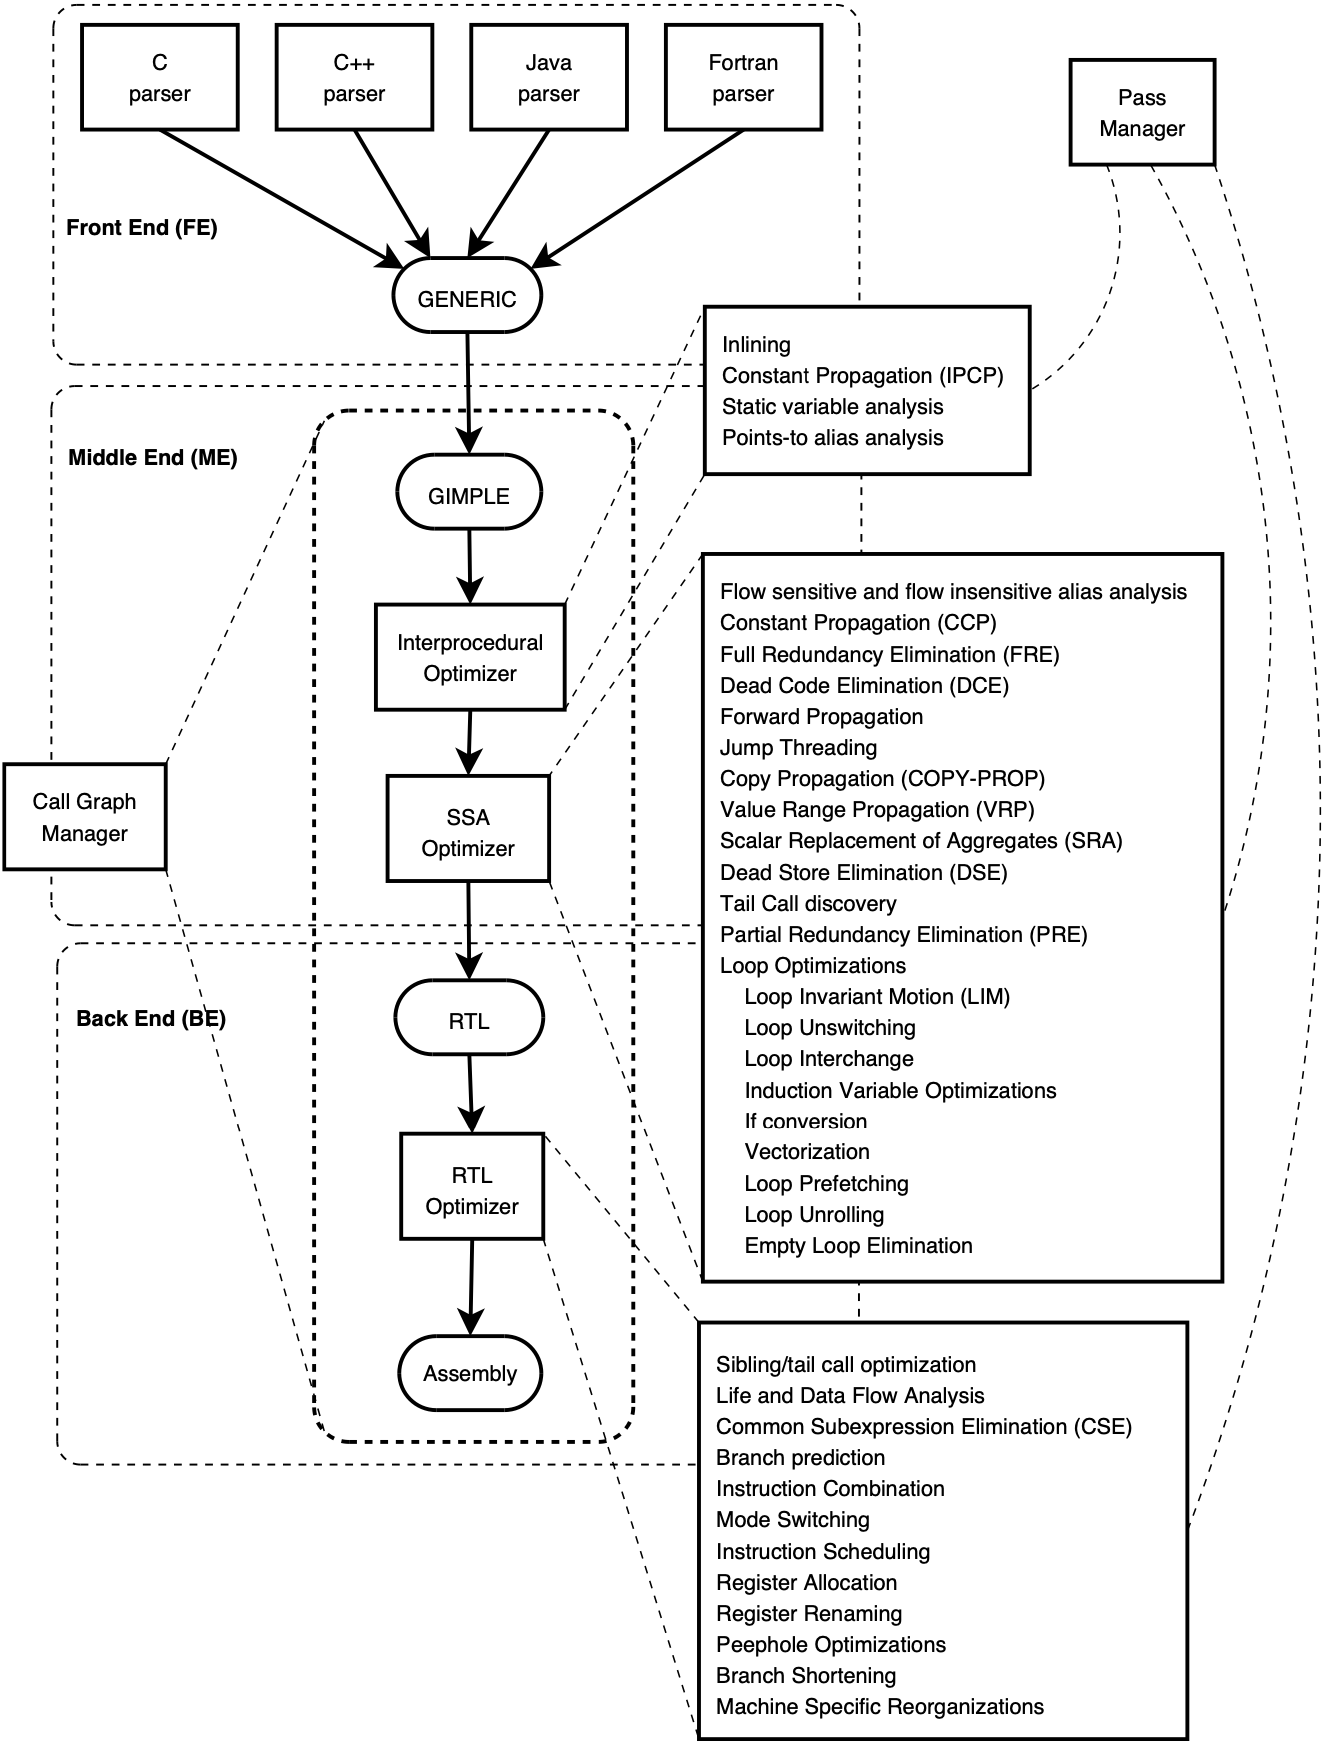
\includegraphics [width=0.95\linewidth]{pictures/GCCoverview.png}
\caption{An Overview of GCC\cite{b1}}
\label{fig1}
\end{figure}

Figure 1 shows a bird's eye view of the compiler. Notably, the various phases are orchestrated by the Call Graph and Pass managers. The call graph manager constructs a call graph for the compilation unit, determining the order in which each function should be processed. Additionally, it facilitates inter-procedural optimizations (IPO), such as inlining. On the other hand, the pass manager oversees the sequencing of individual transformations and manages pre and post cleanup actions required by each pass.

The source code is organized in three major groups: core, runtime and support. In what follows all directory names are assumed to be relative to the root directory where GCC sources live.\cite{b1}

\subsection{Optimization Level}
Typically, optimizations provided by GCC can be divided into three degrees. Some optimizations make the assembly code shorter, while others speed up the code, which potentially is enlarged.

The O1 optimization level in GCC represents a moderate level of compiler optimization designed to enhance program performance while maintaining a relatively swift compilation process. The primary focus is on applying fundamental optimizations to the code. The O1 optimization level strikes a balance between improving program performance and minimizing compilation time, making it suitable for scenarios where moderate optimization is desired without significantly impacting build times. Here are some key aspects of O1 optimization:
\begin{itemize}
	\item Unused Variable Removal:
The compiler identifies and eliminates variables that are declared but not used in the program. This helps reduce the size of the generated code.
	\item Expression Simplification:
O1 includes basic expression simplification, where the compiler aims to simplify complex expressions, potentially leading to more efficient code execution.
	\item Code Layout Optimization:
The compiler may perform basic code layout optimizations, reorganizing code sections to improve locality and potentially enhance runtime performance.
	\item Inlining of Functions:
O1 may include basic function inlining, where small functions are substituted directly into the calling code to reduce the overhead of function calls.
	\item Strength Reduction:
Basic strength reduction techniques may be applied to replace expensive operations with cheaper equivalents, optimizing arithmetic expressions for improved performance.
	\item Control Flow Optimization:
Basic control flow optimizations are employed to simplify and streamline conditional statements and loops, potentially reducing branch mispredictions.
	\item Minimization of Code Size:
While not the primary focus, O1 aims to keep the generated code relatively compact, balancing performance improvements with code size considerations.
\end{itemize}

\begin{figure}[htbp]
\centering
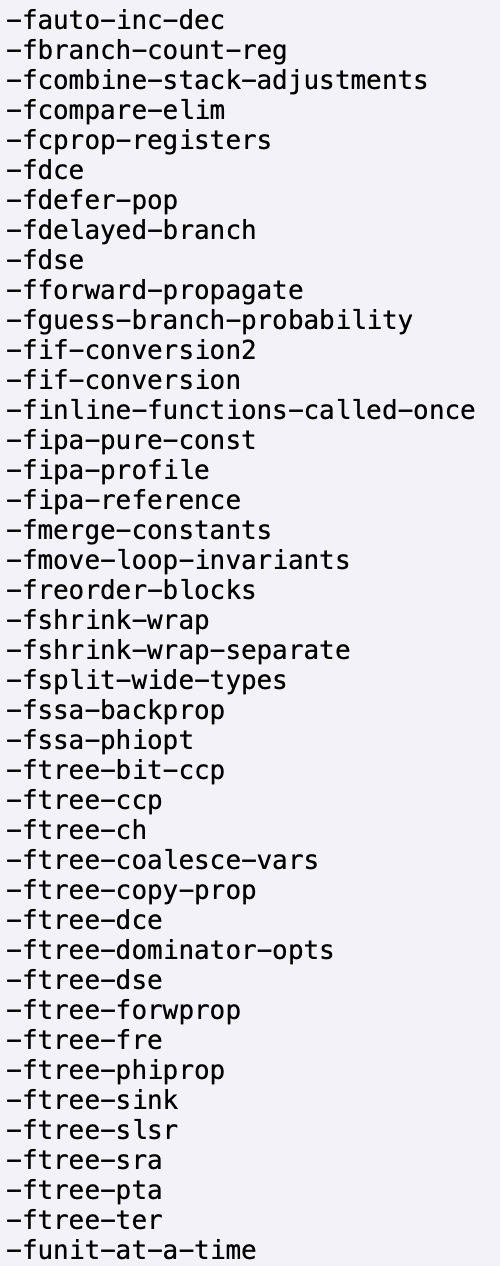
\includegraphics [width=0.4\linewidth]{pictures/o1.png}
\caption{O1 Optimization Flags\cite{b2}}
\label{fig2}
\end{figure}

The O2 optimization level in GCC encompasses a set of advanced compiler optimizations aimed at substantially improving program performance. Building upon the optimizations introduced in O1, O2 introduces more sophisticated techniques. It is characterized by a more aggressive set of optimizations, making it suitable for scenarios where achieving higher performance is a priority, even at the cost of slightly longer compilation times. Below is a detailed description, combining the objectives and impacts:
\begin{itemize}
	\item Loop Unrolling: Replicating loop bodies to reduce loop control overhead and enhance instruction-level parallelism, thereby improving execution speed.
	\item Data Flow Analysis: Analyzing the flow of data through the program facilitates a better understanding of variable relationships, leading to more effective optimizations.
	\item Cross-Module Inlining: Extending function inlining to functions defined in separate compilation units enhances opportunities for inlining across different parts of the program.
	\item Strength Reduction: Replacing expensive operations with cheaper equivalents optimizes arithmetic expressions for improved efficiency.
	\item Loop Fusion: Combining adjacent loops reduces loop overhead, improving cache locality and reducing loop control overhead.
	\item Loop Distribution: Distributing loop iterations enables better parallelization, improving the potential for parallel execution of loop iterations.
	\item Vectorization: Converting scalar operations into vector operations leverages SIMD instructions, enhancing parallelism, especially on architectures with SIMD support.
\end{itemize}

\begin{figure}[htbp]
\centering
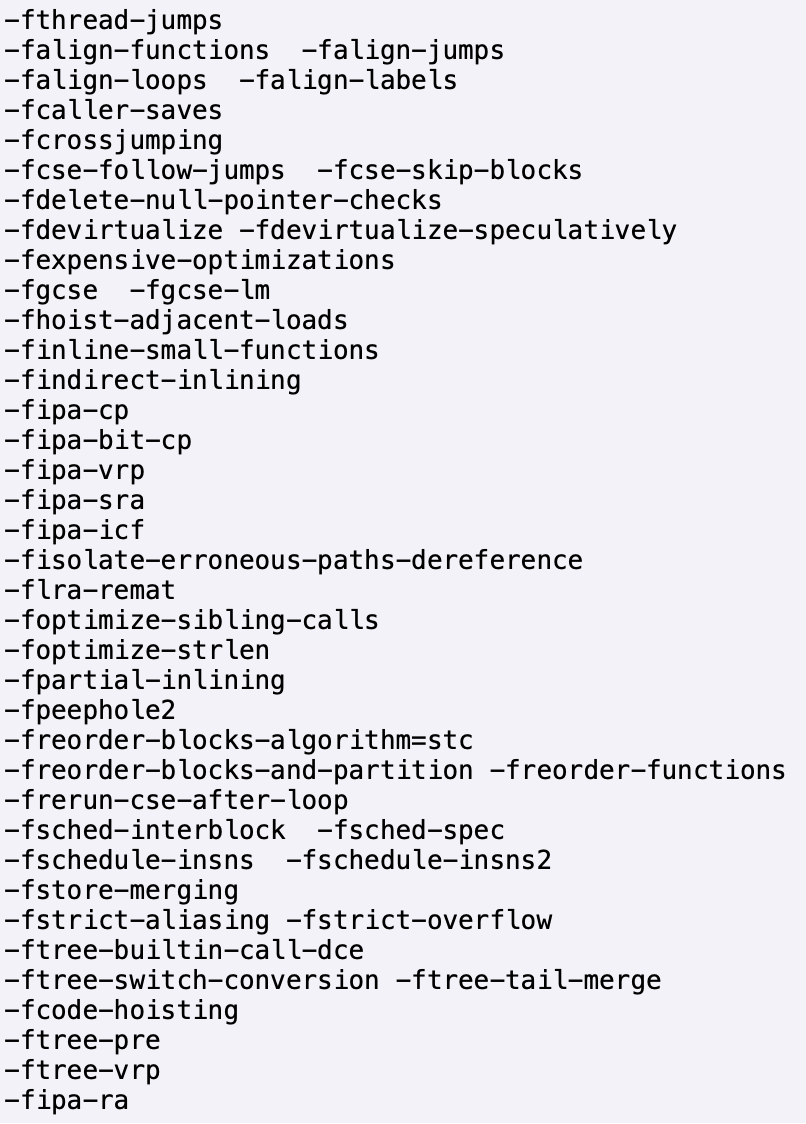
\includegraphics [width=0.7\linewidth]{pictures/o2.png}
\caption{O2 Optimization Flags\cite{b2}}
\label{fig3}
\end{figure}

The O3 optimization level in GCC represents the highest degree of compiler optimization, aimed at maximizing program performance, even if it results in longer compilation times. Building upon the optimizations introduced in O2, O3 incorporates more sophisticated and time-consuming techniques.

While the -O3 optimization level is capable of generating high-performance code, it's important to note that the resulting increase in the size of the executable can potentially have detrimental effects on its speed. Specifically, if the size of the executable surpasses the capacity of the available instruction cache, this could lead to significant performance penalties. Consequently, it might be more prudent to opt for compiling at the -O2 optimization level. This decision is driven by the intention to enhance the likelihood that the executable fits within the constraints of the instruction cache, thereby mitigating the risk of severe performance degradation.

The Os optimization level focuses on minimizing the size of the generated executable. It aims to reduce the overall footprint of the compiled program, making it suitable for environments where compactness is a priority, such as embedded systems with limited storage.

The -Ofast optimization level is similar to -O3 but allows for more aggressive optimizations, including those that may affect mathematical precision. It prioritizes maximizing execution speed and might not be suitable for applications where strict adherence to floating-point precision is required.

To illustrate the impact of GCC compiler optimization levels, we'll use a C code example that performs numerical computations. We'll use a simple numerical integration algorithm as our case study. Below is the code without any optimizations applied:

\begin{figure}[htbp]
\centering
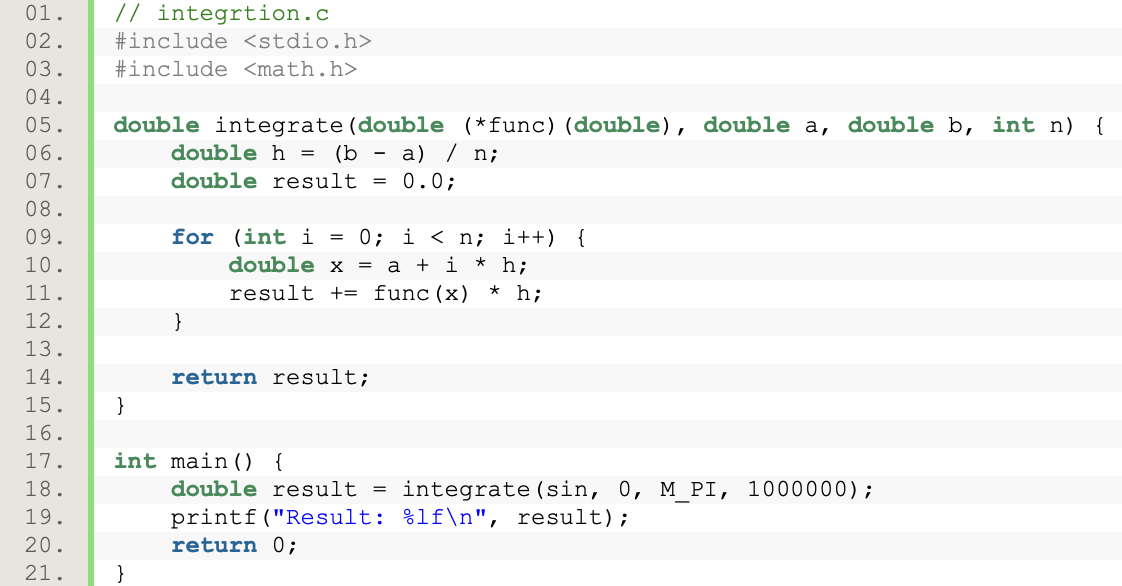
\includegraphics [width=0.9\linewidth]{pictures/gcc_sample_code.png}
\caption{C Code Example that Performs Numerical Computations\cite{b3}}
\label{fig4}
\end{figure}

Running on the same computer, the statistics are shown in Table 1. The "Real" time is the actual wall-clock time it took to execute the program. The "User" time represents the CPU time consumed by the program. The "Sys" time indicates system-related CPU time.\cite{b3}

\begin{table}
	\caption{Running Time}
	\begin{center}
		\begin{tabular}{c c c c c c}
			\toprule
			Optimization &default&O2&O3&Os&Ofast\\
			\hline
			Real & 0.064s & 0.041s & 0.058s & 0.016s & 0.067s\\
			User & 0.064s & 0.041s & 0.058s & 0.015s & 0.066s\\
			Sys  & 0.001s & 0.001s & 0.001s & 0.001s & 0.001s\\
			\bottomrule
		\end{tabular}
	\end{center}
\end{table}

Specifying the target architecture also can yield meaningful benefits. The -march option of gcc allows the CPU type to be specified. The default architecture is i386. GCC runs on all other i386/x86 architectures, but it can result in degraded performance on more recent processors. Let's now look at an example of how performance can be improved by focusing on the actual target. Build a simple test application that performs a bubble sort over 10,000 elements. The elements in the array have been reversed to force the worst-case scenario.\cite{b4}

\begin{figure}[htbp]
\centering
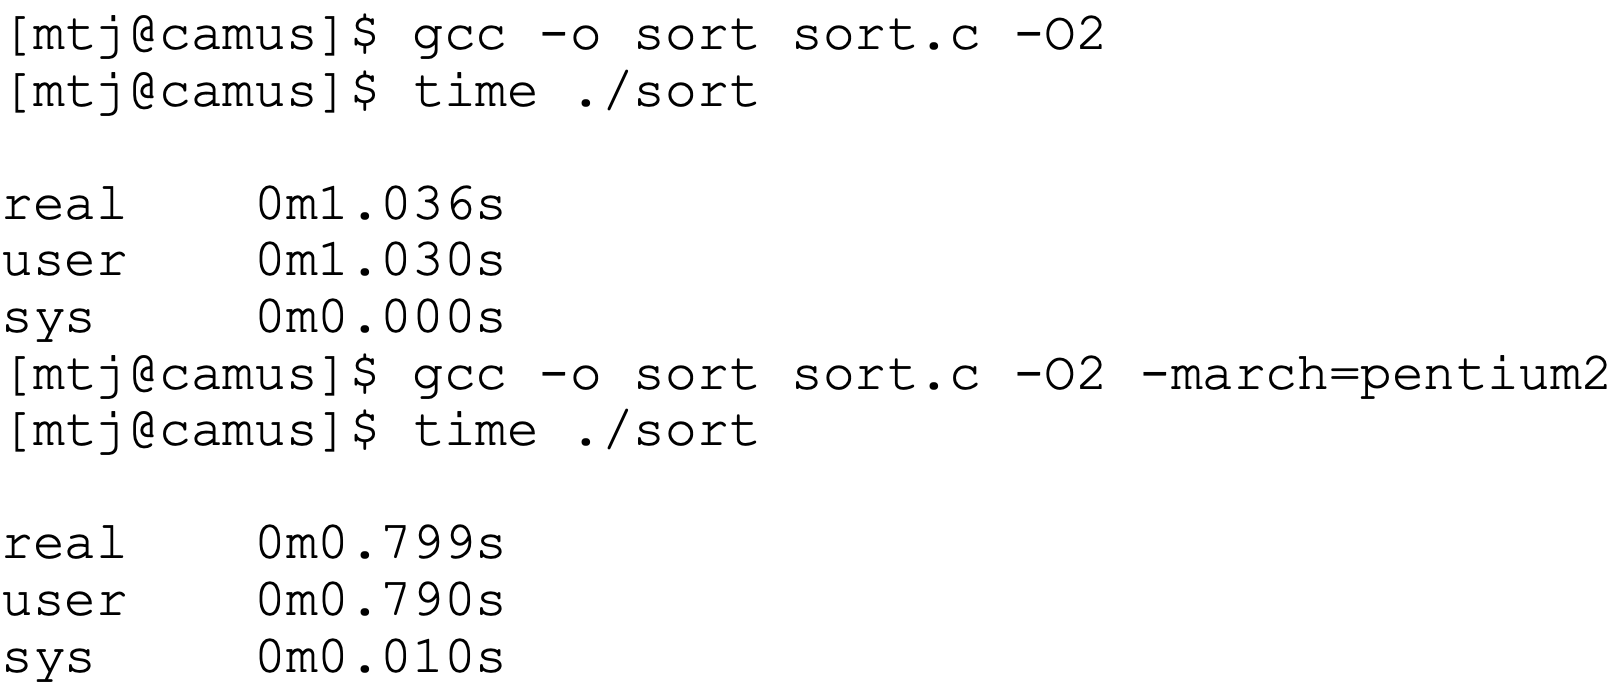
\includegraphics [width=0.85\linewidth]{pictures/GCCarchi.png}
\caption{Effects of Architecture Specification on a Simple Application\cite{b4}}
\label{fig5}
\end{figure}

By specifying the architecture, in this case a 633MHz Celeron, the compiler can generate instructions for the particular target as well as enable other optimizations available only to that target. As shown in Figure 5, by specifying the architecture we see a time benefit of 237ms (23\% improvement). Although it shows an improvement in speed, the drawback is that the image is slightly larger. Using the size command, we can identify the sizes of the various sections of the image.\cite{b4}

\begin{figure}[htbp]
\centering
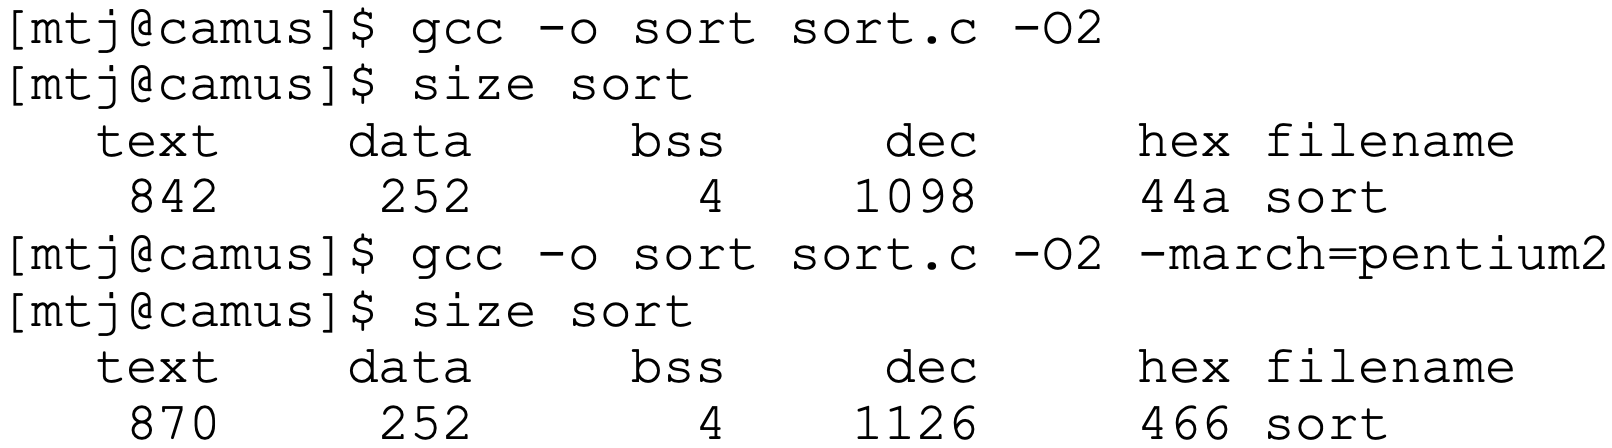
\includegraphics [width=0.85\linewidth]{pictures/GCCsize.png}
\caption{Size Change of the Application\cite{b4}}
\label{fig6}
\end{figure}

Here the instruction size (text section) of the image increased by 28 bytes. But in this example, it's a small price to pay for the speed benefit.\cite{b4}

In conclusion, optimizing your code with GCC is not just a luxury but a necessity in today's demanding software landscape. A profound understanding of the diverse optimization levels and their judicious application can elevate your code to the status of an efficient, high-performing masterpiece.

However, a word of caution is essential. Optimization is akin to a double-edged sword. While it has the potential to deliver remarkable performance gains, it should not come at the expense of the readability and maintainability of your code. Striking the delicate balance between optimization and code quality is an art that every developer must master.

\subsection{Vectorization}

Vectorization in GCC refers to the process of transforming scalar operations within code into vector operations, a technique particularly pertinent to SIMD (Single Instruction, Multiple Data) architectures where a single instruction can concurrently operate on multiple data elements.

The objective of vectorization is to enhance parallelism and harness the capabilities of contemporary processors equipped with vector units. These vector units facilitate the simultaneous execution of a single instruction on multiple data elements, thereby amplifying throughput and overall performance.

In Figure 7, the compiler on the left is capable of computing only one pair of scalar multiplications at a time. Consequently, the multiplication of four pairs of numbers requires four separate operations. Conversely, the compiler on the right possesses the capability to concurrently process four numbers, enabling the completion of the multiplication of four pairs of numbers in a single operation.

\begin{figure}[htbp]
\centering
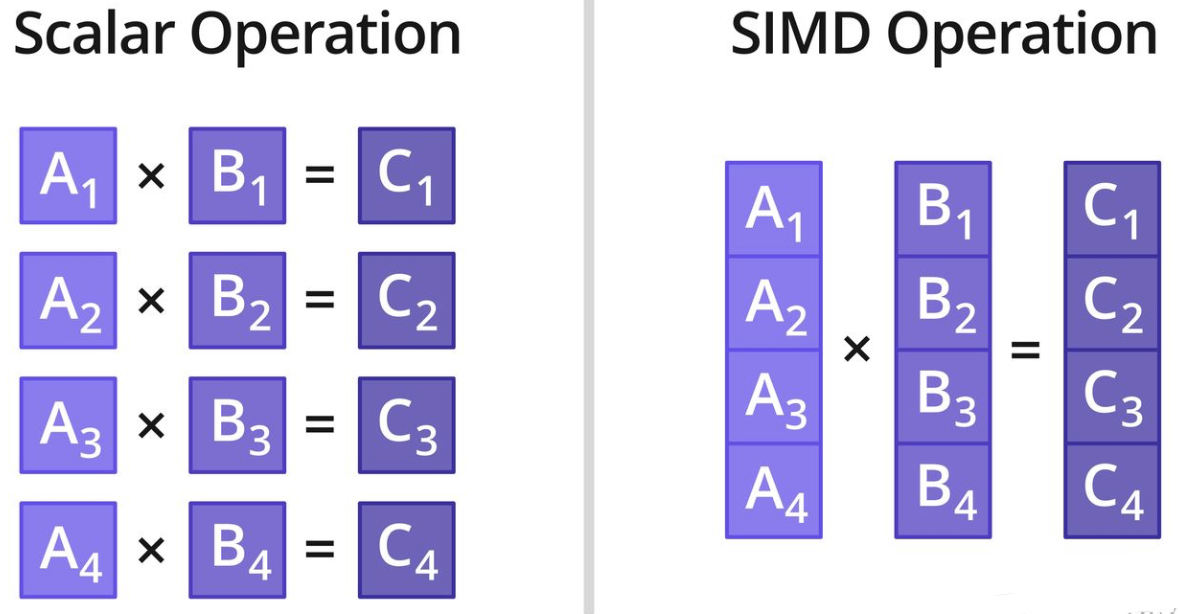
\includegraphics [width=0.8\linewidth]{pictures/SIMD.png}
\caption{A comparison between scalar and SIMD operation\cite{b5}}
\label{fig7}
\end{figure}

In modern computing, SIMD processing units or GPUs are primarily employed for vector processing. High-end CPUs commonly integrate specialized instruction sets for SIMD operations, such as Intel's SSE and AVX. The SIMD processing capability of CPUs operates in a parallel fashion within a single core. The parallel paradigm in multicore processing is referred to as MIMD (multiple instruction multiple data). The distinction lies in SIMD's execution in a lockstep manner, where all ALU units share a single program counter (PC). In contrast, MIMD involves independent execution across cores, each with its own PC.

In GCC, using vector instructions through built-in functions is available. On some targets, the instruction set contains SIMD vector instructions which operate on multiple values contained in one large register at the same time.\cite{b6}

Assuming our SIMD processor can handle $4$ double numbers at once, take an addition of two arrays as an example. Inside the loop in line 14, it loads four single-precision floating-point values from the array $a$ into a Neon vector $va$. Then in adds the loaded vector $va$ element-wise to the cumulative sum vector $vsum$. It accumulates the sum as the loop progresses. After the loop, it uses Neon intrinsics to perform pairwise addition on the lower and higher lanes of the cumulative sum vector $vsum$, resulting in a 2-element vector $sum_lane$. Finally it completes the reduction by adding the two elements of the 2-element vector $sum_lane$. The result is a single-precision floating-point value representing the sum of the vectorized elements.

\begin{figure}[htbp]
\centering
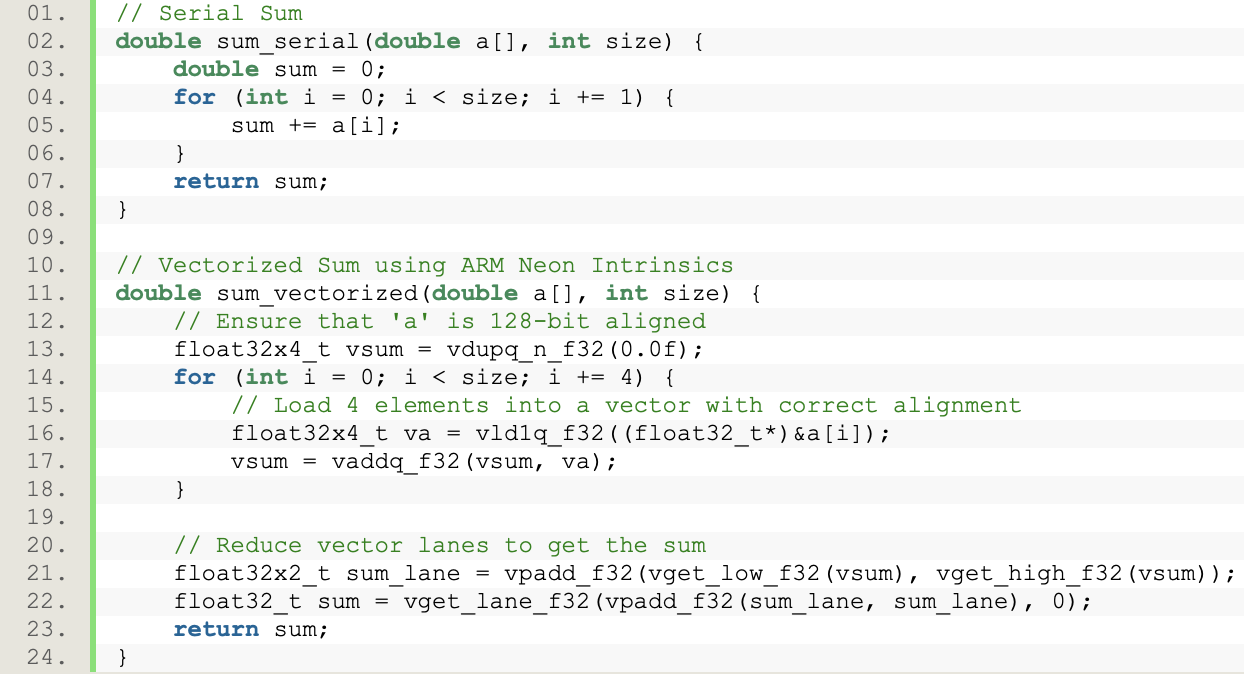
\includegraphics [width=0.95\linewidth]{pictures/SIMD_code.png}
\caption{SIMD Code Example}
\label{fig8}
\end{figure}

When the array size is $100000000$, the serial time and vectorized time is $0.3656$ seconds and $0.1772$ seconds (Apple M2), respectively, which indicates a crucial speedup.

In the context of parallelized numerical accumulation, it is essential to recognize that the order of summation may change due to parallel processing. To achieve parallelism, associativity, the property that allows rearrangement of operands without altering the result (e.g., $a+b+c+d=(a+b)+(c+d))$, becomes crucial. This property ensures that parallel addition remains consistent even with a different summation order.

However, when dealing with floating-point operations involving multiplication or addition, achieving strict associativity can be challenging. Floating-point arithmetic, subject to rounding errors, may not strictly adhere to associativity, especially when parallelized. Consequently, to facilitate parallel floating-point operations, specialized compiler options such as `--ffast-math' in GCC are often employed. These options relax strict adherence to IEEE standard compliance and allow for more aggressive optimizations.

Maintaining numerical stability in the face of reordering operations for parallelism is a fundamental concern. Rounding errors, inherent in floating-point calculations, can accumulate differently depending on the order of operations. Achieving both parallelism and numerical stability requires a delicate balance. The use of appropriate compiler flags, careful algorithm design, and consideration of numerical stability principles are essential in minimizing the impact of rounding errors and ensuring reliable parallel computations.

\subsection{Back-end Optimization Analysis}

Register Transfer Language (RTL) is a crucial intermediate representation in the context of compiler construction, serving as a pivotal bridge between high-level source code and low-level machine code within the framework of GCC. The RTL generation, optimization, and assembly code generation processes constitute an intricate series of stages aimed at transforming abstract program structures into efficient machine-executable instructions.

The RTL generation process involves the translation of the abstract syntax tree (AST) derived from the high-level source code into a hardware-oriented, register-transfer-based representation. This step captures the essential data and control flow aspects of the program, representing them in terms of RTL operations and their associated operands. This intermediate form serves as a foundation for subsequent analyses and transformations.

RTL optimization encompasses a suite of techniques geared toward enhancing the performance of the generated code. This involves a myriad of low-level optimizations such as register allocation, instruction scheduling, and dead code elimination. Register allocation seeks to judiciously assign program variables to processor registers, minimizing memory accesses and improving overall execution speed. Instruction scheduling aims to reorder operations to exploit parallelism and reduce pipeline stalls. Additionally, dead code elimination identifies and removes code segments that contribute no discernible impact on program output.

Subsequent to RTL optimization, the compiler proceeds to the generation of assembly code tailored to the target architecture. This involves mapping RTL operations and operands to specific machine instructions, considering the intricacies of the underlying hardware. The assembly code generated at this stage serves as the final output that can be further processed by an assembler to produce machine code executable on the target platform.

The processes of RTL generation, optimization and assembly code generation, should be guided by machine description. The machine descriptions are composed of three files: target machine-description macro definitions file (target.h), machine-description functions support file (target.c) and target machine descriptions file (target.md).\cite{b7}

These descriptions play a pivotal role in the backend stages of the compiler, particularly during the code generation phase. Compiler utilization of machine descriptions ensures the generation of assembly code congruent with the target machine architecture. These descriptions not only furnish the compiler with the requisite information for the production of correct code but also endow the optimizer with insights, facilitating the adept utilization of the target machine's features to enhance code performance.

\begin{figure}[htbp]
\centering
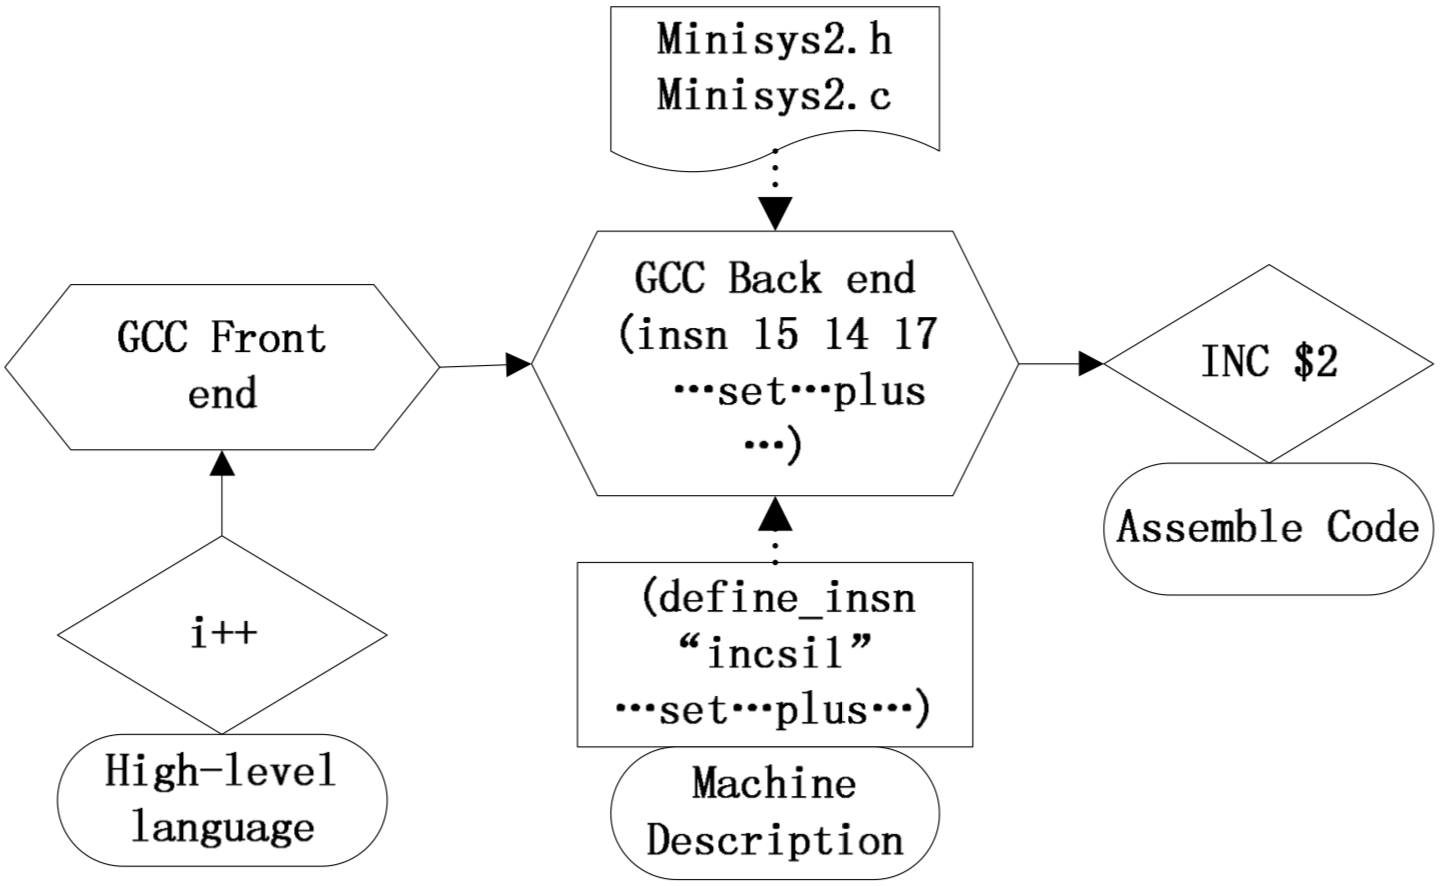
\includegraphics [width=0.95\linewidth]{pictures/i++.png}
\caption{Example Code `i++' Compilation Process\cite{b7}}
\label{fig9}
\end{figure}

It deserves to be mentioned that the efficiency of complier should be taken into full account in the porting process. As the pattern of each instruction is matched in order, the more instruction patterns there are, the more slowly the compiling system will be. It is better to combine the similar instructions to one instruction pattern to obtain higher complier efficiency. The priority of instruction matching should be paid attention to at the same time. Take a simple C language sentence `i++' as an example and set the target machine as Minisys2. The result of matching can be `INC \$2', as well as the mode of `add \$2, \$3, 1'. The process of matching `target.md' file is carried out through the order from top to bottom in GCC, so `INC' instruction pattern should be put in the front of `add' instruction pattern in order to test the newly increased “INC” instruction.\cite{b7}

In summation, machine descriptions serve as crucial metadata in the compiler domain, delineating how the compiler interfaces with a specific target architecture, thereby enabling the production of accurate and efficient machine code.

\subsection{Summary of GCC}

GCC plays a pivotal role in the entire process of translating source code into target machine executable code. Its impact extends across critical facets of software development.

The primary function of GCC lies in the transformation of source code, authored in high-level programming languages such as C and C++, into executable code for the target machine. It accommodates various target architectures, enabling developers to create and execute programs on diverse platforms.

As an open-source and widely adopted compiler, GCC has exerted a profound influence on the entire software ecosystem. It affords developers the capability for cross-platform development, fostering software portability. Furthermore, the existence of GCC has propelled advancements in compiler technology, serving as a template for numerous other compiler projects.

GCC incorporates a potent optimizer capable of enhancing the performance of the generated target code during the compilation process. Optimization spans various dimensions, encompassing, but not limited to, constant folding, register allocation, instruction scheduling, and loop optimization. Through these optimization techniques, GCC generates machine code that is not only more efficient but also aligns closely with the underlying hardware capabilities.

\begin{thebibliography}{00}

	\bibitem{b1} Novillo, D. (2006, September). GCC an architectural overview, current status, and future directions. In Proceedings of the linux symposium (Vol. 2, p. 185).
	\bibitem{b2} GNU Compiler Collection. (2017). Optimize Options. GNU Compiler Collection Documentation. Retrieved from https://gcc.gnu.org/onlinedocs/gcc-7.2.0/gcc/Optimize-Options.html
	\bibitem{b3} Bharatiya, P. (2023, November 1). Maximizing C++ Program Performance: A Comprehensive Guide to GCC Compiler Optimization. Data Intelligence. Retrieved from https://data-intelligence.hashnode.dev/maximizing-c-program-performance-a-comprehensive-guide-to-gcc-compiler-optimization
	\bibitem{b4} Jones, M. T. (2005). Optimization in GCC. Linux journal, 2005(131), 11.
	\bibitem{b5} Qingyang CHEN. (2023, November 9). Retrieved from https://zhuanlan.zhihu.com/p/337756824
	\bibitem{b6} GNU Compiler Collection. Vector Extensions. GNU Compiler Collection Documentation. Retrieved from https://gcc.gnu.org/onlinedocs/gcc/Vector-Extensions.html
	\bibitem{b7} Xiaowei, W., Kuixing, W., Quansheng, Y. (2012). Research and Development of Compiler Based on GCC. Recent Advances in Computer Science and Information Engineering: Volume 3, 809-814.

\end{thebibliography}


\vspace{12pt}
\end{document}
